\chapter[Elementary Concepts]{Elementary Concepts of Discrete
Dynamical Systems}

\section{Orbits}

% \shadowbox{\url{http://aix1.uottawa.ca/~bdionne}} or
% \shabox{\url{http://aix1.uottawa.ca/~bdionne}}, that is the question?

\begin{defn} \index{Orbit}
Consider $f:\RR \rightarrow \RR$ and $x \in \RR$.  The
{\bfseries forward orbit}\index{Orbit!Positive orbit} of $x$ is the set
\[
\OO^+ = \left\{ x, f(x), f^2(x) = f(f(x)), f^3(x)= f(f(f(x))), \ldots
\right\} \ .
\]
\nomenclature{$\OO^+$}{Positive orbit}
If $f$ has an inverse $f^{-1}:\RR\rightarrow \RR$, the
{\bfseries backward orbit}\index{Orbit!Negative orbit} of $x$ is the set
\[
\OO^- = \left\{ x, f^{-1}(x), f^{-2}(x) = f^{-1}(f^{-1}(x)),
f^{-3}(x)= f^{-1}(f^{-1}(f^{-1}(x))), \ldots \right\}
\]
\nomenclature{$\OO^-$}{Negative orbit}
and the orbit of $x$ is $\OO = \OO^+ \cup \OO^-$.
\nomenclature{$\OO$}{orbit}
\end{defn}

\begin{defn}
Consider $f:\RR \rightarrow \RR$ and $x \in \RR$.  $x$ is a
{\bfseries periodic point}\index{Periodic point} of $f$ if there
exists a positive integer
$n$ such that $f^n(x) = x$.  If $n$ is the smallest positive integer
such that $f^n(x)=x$, we say that $x$ is of {\bfseries period} $n$.
When $n=1$, $x$ is a {\bfseries fixed point}\index{Fixed point}.  We denote by
$\Per_n(f)$ the set of all periodic point of $f$ of period $n$.  In
particular, $\Fix(f) = \Per_1(f)$ is the set of fixed points of $f$.
If $x$ is a periodic point of $f$, $\OO^+$ is a
{\bfseries periodic orbit}.
\nomenclature{$\Per_n(f)$}{Periodic point of period $n$}
\end{defn}

If the mapping $f$ in the previous definition is differentiable (or is
a diffeomorphism), a local stability analysis can be performed to
determine the behavior of orbits around periodic orbits.  More on this
subject later.

\begin{egg}
Consider the {\bfseries logistic map}
\[
f_\mu(x) = \mu x(1-x)
\]
for $0\leq x \leq 1$.  For $0 \leq \mu \leq 4$,
$f_\mu:[0,1]\rightarrow [0,1]$ and $f_\mu$ has two fixed
points: $x=0$ and $x  = \frac{\mu-1}{\mu}$.

For $\mu=3.4$, $x= 0.45195878844045\ldots$ is a periodic point of
$f_\mu$ of period $2$.  The orbit of period two is
\[
\left\{ 0.45195878844045, 0.84215476876273, 0.45195878844045,
0.84215476876273, \ldots \right\} \ ,
\]
where the values have been chopped to $14$ digits after the decimal
point.  This can be easily seen from the {\bfseries graphical
iteration} or {\bfseries cobweb} of $f_\mu$ shown in
Figure~\ref{figCW}.

\begin{figure}
\begin{center}
  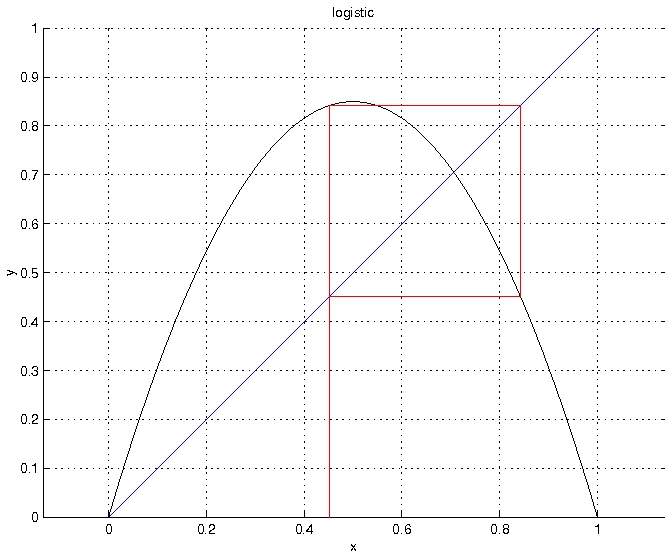
\includegraphics[height=6cm, width=6cm]{logistic1}
\end{center}
\caption[Cobweb]{Cobweb of a discrete dynamical system\label{figCW}}
\end{figure}

For $\mu=3.5$, $x= 0.87499726360246\ldots$ is a periodic point of
$f_\mu$ of period $4$.  The orbit of period four is
\[
\left\{0.87499726360246, 0.38281968301732, 0.82694070659144,
0.50088421030722, \ldots \right\} \ ,
\]
where the values have been chopped
to $14$ digits after the decimal point (Figure~\ref{figPF}).

\begin{figure}
\begin{center}
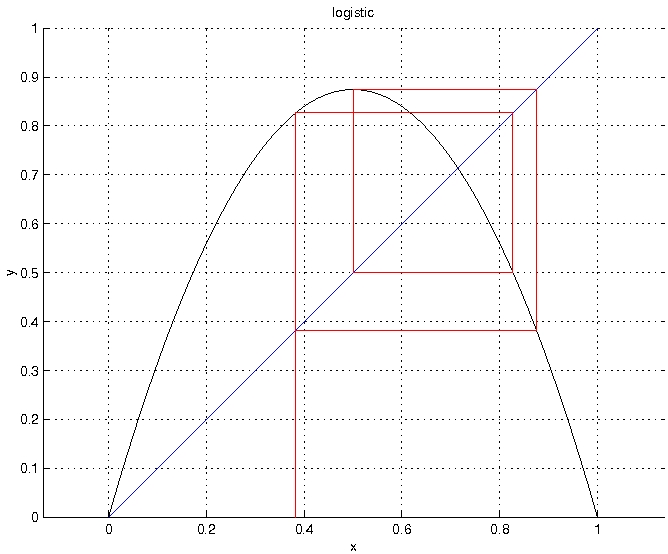
\includegraphics[height=6cm, width=6cm]{logistic2}
\end{center}
\caption[Orbit of Period Four]{Orbit of Period Four\label{figPF}}
\end{figure}
\end{egg}


\begin{proof}[Proof of Theorem X]
  There is noting to proof since it does not exist.   This ilustrate
  how to modify the heading of a proof.
\end{proof}

\begin{proof}
  This proof end with an equation.  So, the \qed\quad has to be properly
  positioned with the use of \verb=\qedhere= at the end of the equation.
  \[
    \frac{1}{\sqrt{2\pi}} \int_0^{2\pi} |f(x)|^2 \text{d}x
    = \sum_{n\in\mathbb{Z}} |\hat{f}(n)|^2  \ .  \qedhere
  \]
\end{proof}

\vfill

%%% Local Variables: 
%%% mode: latex
%%% TeX-master: "template"
%%% End: 
